\section{Introducción}
En la Facultad de Ciencias Físicas y Matemáticas de la Universidad de Chile, ubicada en Santiago, se encuentran dos radiotelescopios, los cuales se encuentran conectados entre sí, formando un interferómetro.\\
\\
\textbf{¿Qué es un interferómetro?}\\
Un interferómetro es un arreglo de dos o más telescopios del mismo tipo (es decir, o telescopios ópticos o radiotelescopios) conectados mediante la técnica de interferometría.\\
La técnica anteriormente mencionada es utilizada para generar un telescopio de gran diámetro separando los telescopios que componen al arreglo en cuestión. En el caso que analizaremos en este informe (es decir, un arreglo compuesto por dos radiotelescopios) se unen las señales obtenidas de cada antena mediante programas computacionales, estableciendo un desfase de periodo en una de las señales para que se simule la curvatura de una parábola propia de una antena de radioastronomía.\\
\\
A lo largo de este informe utilizaremos los espectros obtenidos con dicho interferómetro para calcular el diámetro angular del Sol.\\
El interferómetro cuenta con dos antenas de 2.3 metros de diámetro separadas por aproximadamente $B=37.85$ metros en la dirección Este-Oeste y $\alpha=85.2°$ respecto al norte geográfico. Las antenas estuvieron recibiendo espectros de la temperatura de la antena en Kelvin el año 2011, los días:
\begin{itemize}
    \item 16 de noviembre, entre las 14:40:51 y 23:19:33 hrs, y
    \item 17 de noviembre entre las 09:38:16 y 15:12:11 hrs
\end{itemize}
\\
Para analizar los datos que se obtuvieron, se realizaron los siguientes pasos, en orden:
\begin{enumerate}
    \item Separar los datos en dos (día y noche).
    \item Promediar los espectros obtenidos en los 64 canales.
    \item Filtrar los espectros con cinco métodos distintos.
    \item Obtener una expresión para la apertura $B_s$. Este dato corresponde a la proyección de la separación entre ambas antenas en el frente de onda plano (en función del azimut y la elevación de la fuente).
    \item Realizar un ajuste con un modelo de visibilidad del Sol para un interferómetro de dos antenas con un modelo del Sol de disco plano.
\end{enumerate}
A partir del ajuste mencionado se obtuvo que el diámetro angular del Sol fue de $0.45°$ en la mañana y $0.62°$ en la tarde, promediando $0.535°$.
\newpage

\section{Desarrollo y resultados}
\subsection{Marco Teórico}
\begin{figure}[H]
\centering
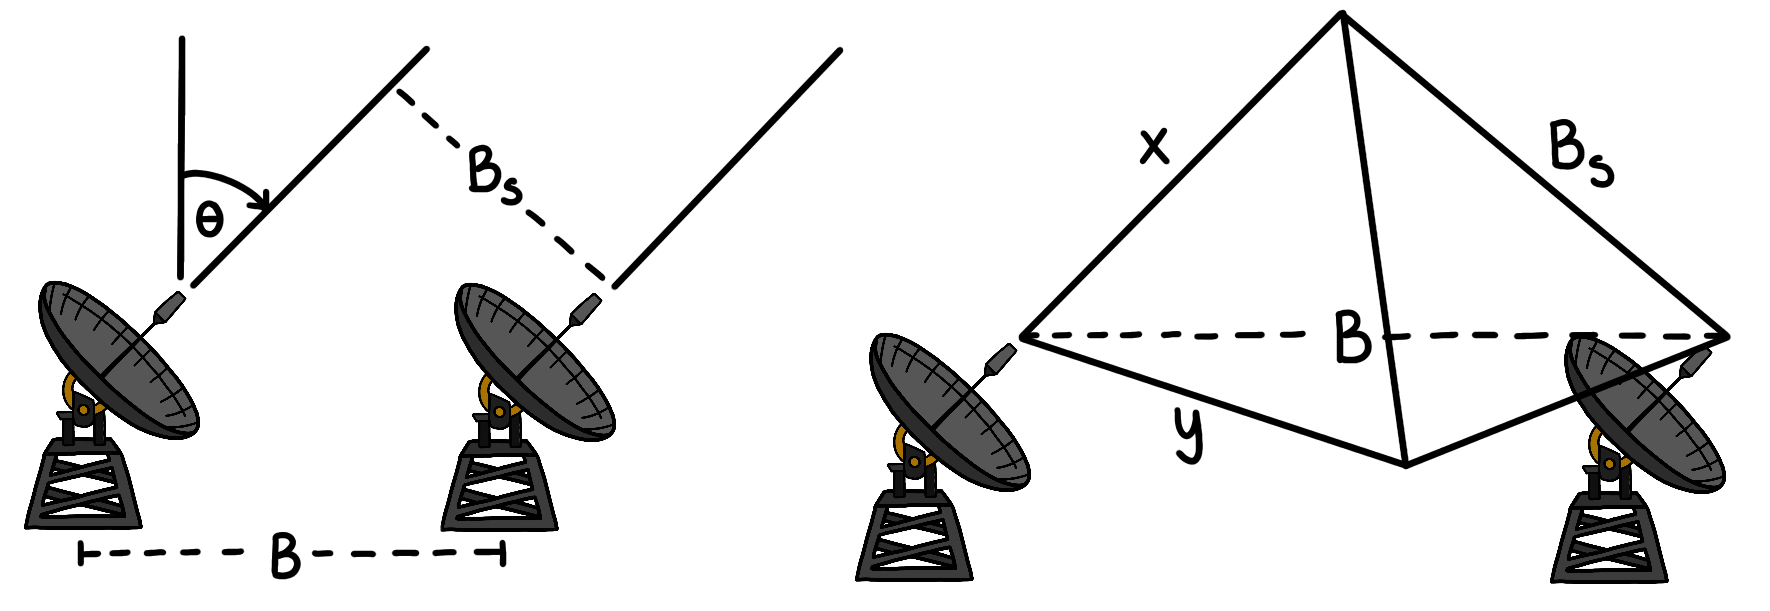
\includegraphics[scale=0.4]{img/img/imagen1.png}
\caption{\label{fig:Grafico} Geometría de un interferómetro de dos antenas}
\end{figure}
Aplicando geometría a la Figura 1 se obtiene la expresión (1) para la apertura $B_s$
\begin{equation}
    B_s=B\sqrt{1-cos^2(azim-\alpha)cos^2(el)}
\end{equation}
Es importante destacar que se trabaja con radianes, por lo que $\alpha$ se traduce de grados sexagesimales a radianes.\\
Posteriormente, se calcula la función de visibilidad $V$, la cual se obtiene tal como indica la ecuación (2)
\begin{equation}
    V=\int\int I(\Omega)P(\Omega)d\Omega
\end{equation}
Donde $P(\Omega)$ es el patrón de radiación y es igual a $cos\left(\frac{2\pi B}{\lambda}cos(\theta)\right)$ e $I(\theta)$ es el brillo. Se considera un brillo constante $I(\theta)=I$. Además, se parametriza el disco solar como $x^2+y^2=R^2$, con $R$ el radio angular del Sol.\\
Lo anterior da como resultado para la visibilidad en función del diámetro angular del Sol la ecuación (3).
\begin{equation}
    V(d)=\abs{\frac{sin(\pi B_s d)}{\pi B_s d}}
\end{equation}
\subsection{Resultados}
Cada medición se realizó en 64 canales, por lo cual para obtener el espectro promedio se realizó un promedio de cada medición pasando por los 64 canales. Se estableció un límite entre 1 000 y 6 000 en el eje de las ordenadas, para poder observar de mejor manera el resultado.
\begin{figure}[H]
\centering
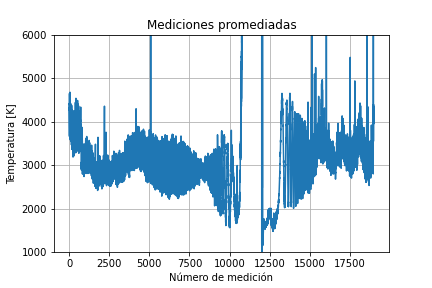
\includegraphics[scale=0.55]{img/img/inf4graf1.png}
\caption{\label{fig:Grafico} Mediciones promediadas}
\end{figure}
Se separaron las mediciones entre la mañana y la tarde. Nuevamente se promediaron las mediciones pasando por los 64 canales y se estableció el mismo límite en el eje de las ordenadas.\\
En este punto aún no se realiza ningún filtro al espectro.
\begin{figure}[H]
\centering
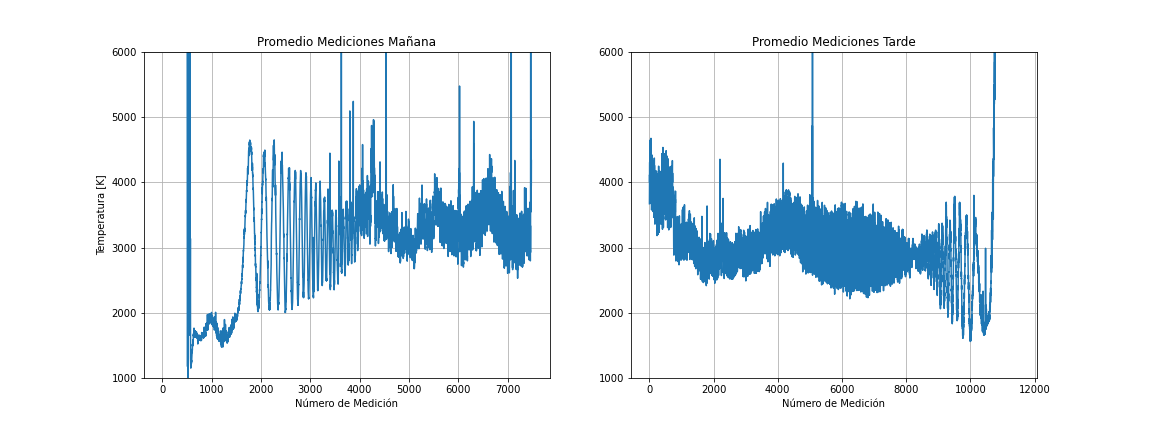
\includegraphics[scale=0.4]{img/img/inf4graf2.png}
\caption{\label{fig:Grafico} Mediciones promediadas separadas por tramo horario}
\end{figure}
A partir de este punto todos los gráficos del informe se separarán por tramo horario para un mejor análisis.\\
Se observa que en ambos gráficos hay conjuntos de mediciones consecutivas que no tienen sentido, para ello se eliminan:
\begin{itemize}
    \item en la mañana, las mediciones 1 a 1 700, y
    \item en la tarde, las mediciones 10 001 en adelante
\end{itemize}
\begin{figure}[H]
\centering
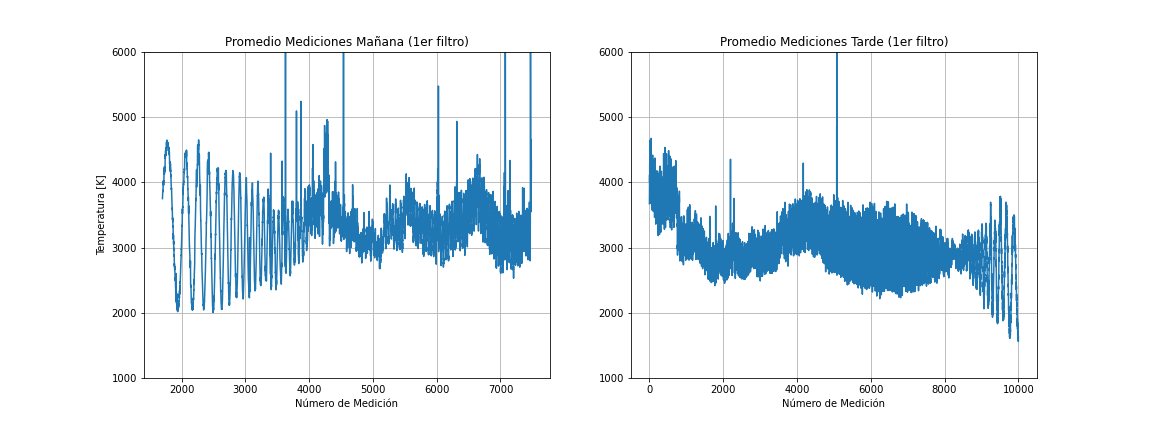
\includegraphics[scale=0.4]{img/img/inf4graf3.png}
\caption{\label{fig:Grafico}: Mediciones tras el primer filtrado}
\end{figure}
Se realiza un filtrado en los datos, manteniendo todos aquellos que no superen la mitad de la RMS (media cuadrática) para cada tramo. Se puede observar que esto elimina aquellas temperaturas exageradamente altas, que no podrían ser reales puesto que la temperatura en la superficie del Sol es de 5 788 K.\\
Se recuerda que la fórmula del RMS es
$$RMS=\sqrt{\frac{1}{n}\sum\limits_i x_i^2}$$
donde $n$ es la cantidad de datos y $x_i$ es el valor de cada dato.
\begin{figure}[H]
\centering
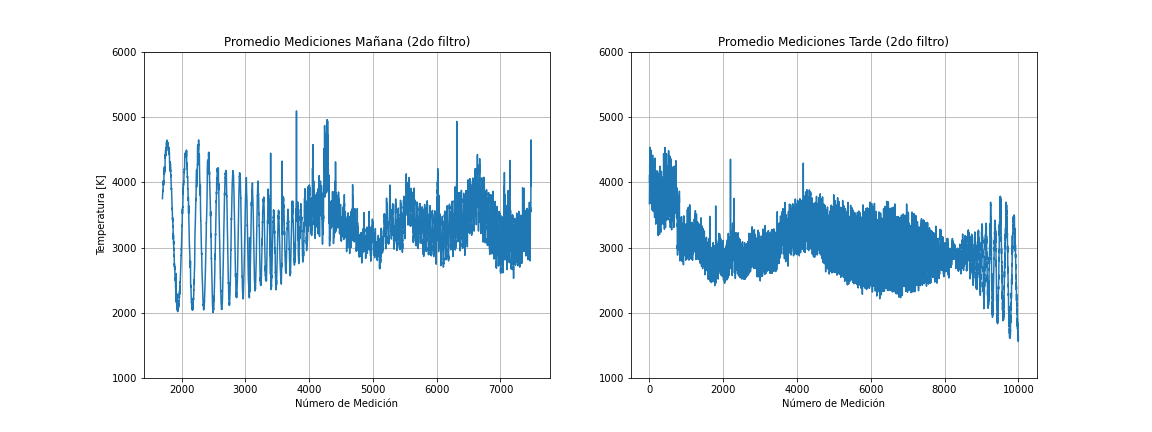
\includegraphics[scale=0.4]{img/img/inf4graf4.png}
\caption{\label{fig:Grafico} Mediciones tras el segundo filtrado}
\end{figure}
Luego, se realiza un filtro de mediana, para eliminar aquellos que, pese a los dos filtrados anteriores, siguen teniendo una subida y posterior bajada brusca.\\
Se aplicó un filtro de mediana de dimensión 9. El algoritmo recorre toda la lista de datos dividiéndola en subconjuntos de 9 datos consecutivos, ordenándola de menor a mayor y seleccionando el dato central (mediana) en el caso de aquellos datos que no tengan sentido, los cuales se infiere que es una interferencia.
\begin{figure}[H]
\centering
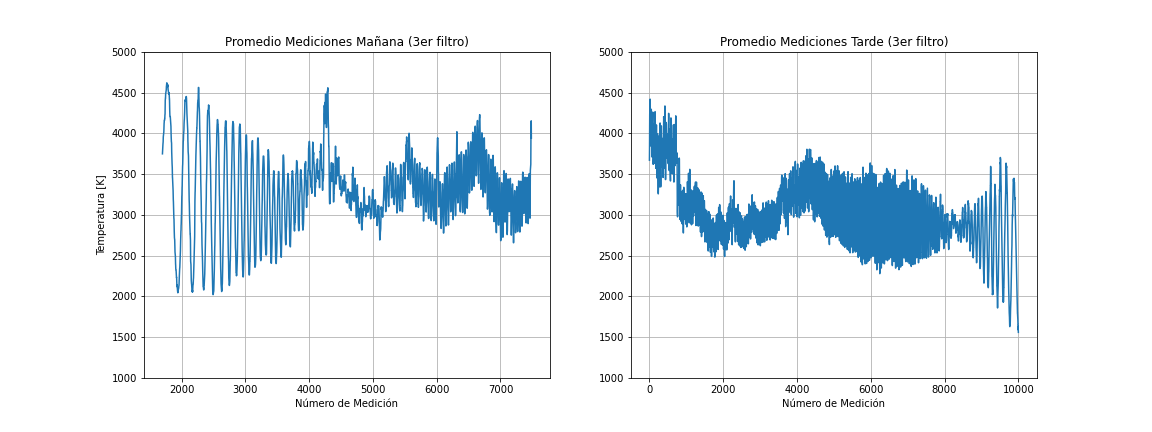
\includegraphics[scale=0.4]{img/img/inf4graf5.png}
\caption{\label{fig:Grafico} Mediciones tras el tercer filtrado}
\end{figure}
Posterior a los tres filtros anteriores, se utiliza la transformada de Fourier (y posteriormente la antitransformada) para centrar los datos en cero.\\
En la Figura 7 se observa la transformada de Fourier aplicada al conjunto de datos luego del filtro de mediana.
\begin{figure}[H]
\centering
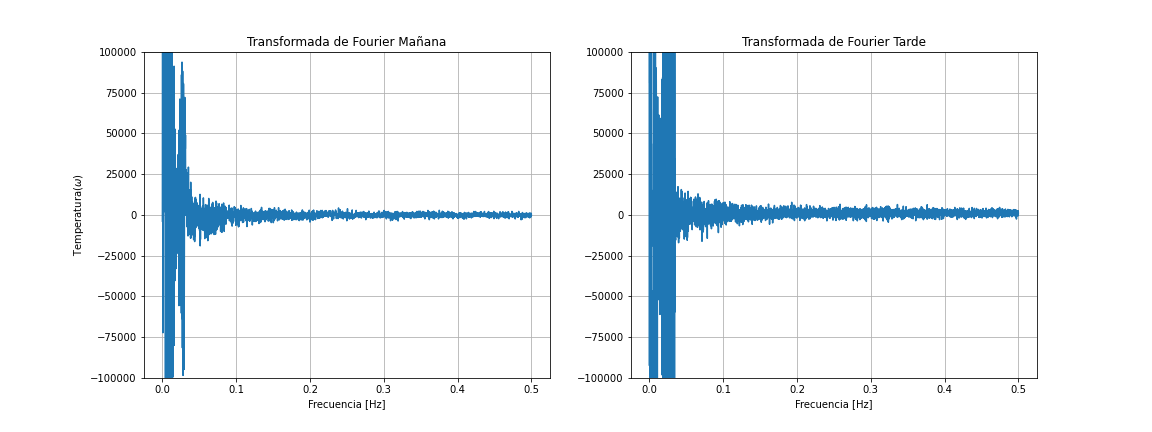
\includegraphics[scale=0.4]{img/img/inf4graf6.png}
\caption{\label{fig:Grafico} Transformada de Fourier de las mediciones}
\end{figure}
Se puede observar que a partir de, aproximadamente, 0.04 [Hz] solo hay ruido y que entre 0 y 0.003 [Hz] no se observan casi datos. Por lo anterior, todos los datos en esos rangos se igualan a cero. En la Figura 8 se observa la transformada filtrada.
\begin{figure}[H]
\centering
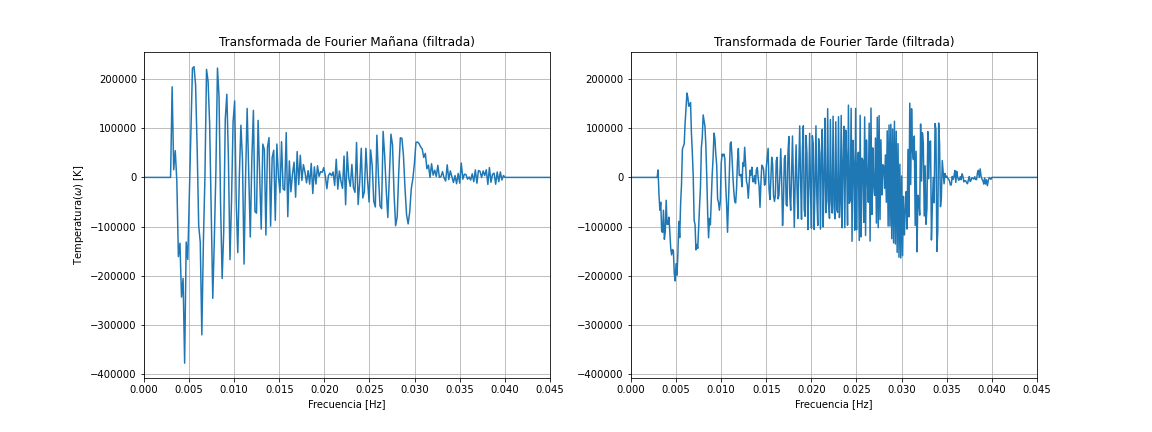
\includegraphics[scale=0.4]{img/img/inf4graf7.png}
\caption{\label{fig:Grafico} Transoformada de Fourier filtrada}
\end{figure}
Posteriormente, se aplica la antitransformada para volver a trabajar con un plano Número de Medición vs. Temperatura [K], obteniéndose el siguiente gráfico. Se observa que las mediciones están centradas en cero. Cabe destacar que este gráfico solo resulta útil para los siguientes pasos, pues no existen temperaturas bajo el cero absoluto (0 [K]).
\begin{figure}[H]
\centering
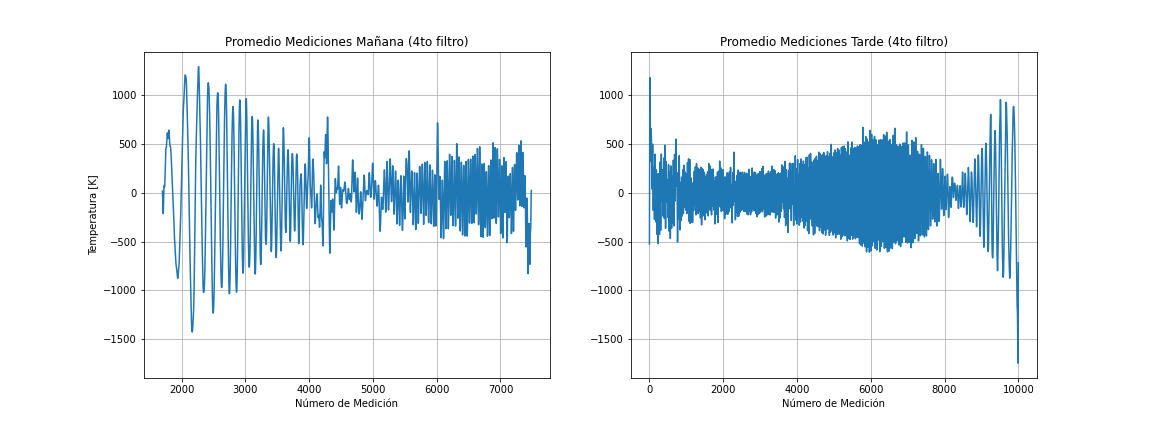
\includegraphics[scale=0.4]{img/img/inf4graf8.png}
\caption{\label{fig:Grafico} Mediciones tras el cuarto filtrado}
\end{figure}
Se calcula la apertura a partir de $B$, el azimut y la elevación. En la Figura 10 se ve la apertura en función del número de mediciones.
\begin{figure}[H]
\centering
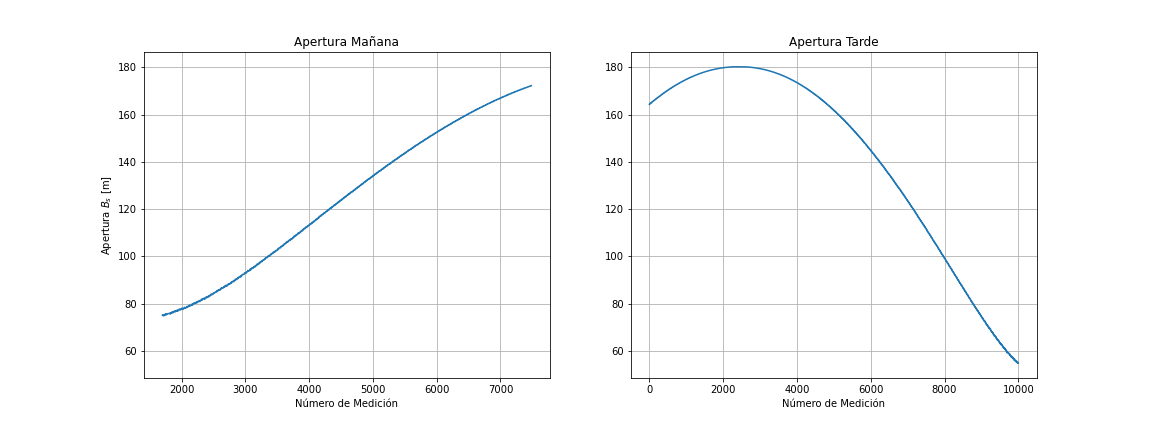
\includegraphics[scale=0.4]{img/img/inf4graf9.png}
\caption{\label{fig:Grafico} Apertura de las mediciones}
\end{figure}
Finalmente, se grafica el valor absoluto de las temperaturas en función de la apertura. Dentro del mismo gráfico se plotea el ajuste en función de la visibilidad.
\begin{figure}[H]
\centering
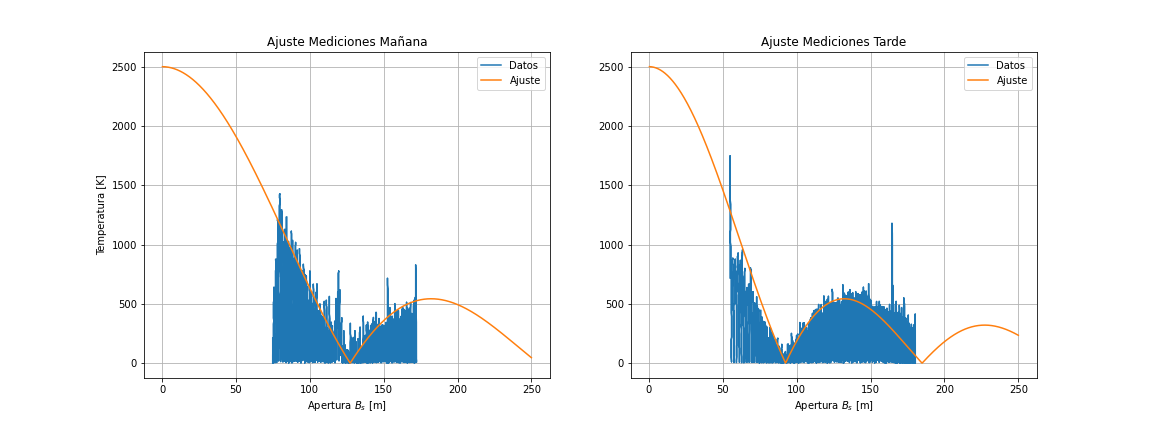
\includegraphics[scale=0.4]{img/img/inf4graf10.png}
\caption{\label{fig:Grafico} Ajuste realizado a las mediciones}
\end{figure}
A partir del ajuste anterior se obtiene que el diámetro angular del Sol en la mañana es 0.45° y en la tarde es 0.62°, promediando 0.535°.
\newpage

\section{Análisis y Conclusiones}
Se observa que el valor obtenido para el diámetro angular del Sol (0.535°) se acerca mucho al esperado de manera analítica (0.53°), lo cual indica que el trabajo realizado en este informe es correcto.\\
\indent Sin embargo, es fácil notar que el diámetro obtenido para los datos de la mañana (0.45°) difiere considerablemente de aquellos de la tarde (0.62°). Esto podría deberse a que no se realizaron mediciones seguidas durante 24 horas y que tanto durante el 16 como el 17 de noviembre se tomaron mediciones entre las 14:40:51 y 15:12:11, lo cual implica repetir datos bastante similares entre sí en ambos espectros. Además, se pueden haber perdido varios datos útiles al momento de realizar los filtrados. A esto se suma la contaminación electromagnética del lugar donde se ubican las antenas (un lugar muy poblado, donde pueden colaborar en esta contaminación ondas de televisión, radio, entre otras).\\
\indent Posteriormente, se compara el diámetro angular del Sol con el main beam, haciendo uso de la ecuación (4)
\begin{equation}
    \theta_{arc}=\frac{2\lambda\ [cm]}{D\ [m]}
\end{equation}
\indent Para una sola antena se obtiene $\theta_{arc}=18\ 347$, es decir $5.1°$. Mientras que considerando el interferómetro se obtiene $\theta_{arc}=1\ 145$, es decir $0.03°$. Debido a lo anterior, se concluye que la técnica de interferometría es más efectiva.\\
La principal limitante del método de la interferometría es que el cielo no se observa de manera uniforme, por lo cual el procesamiento de los datos es mucho más complicado que para una sola antena.\\
\indent A partir de lo anterior, se puede concluir que el método de interferometría es efectivo para realizar investigaciones. Además, es muy conveniente a nivel económico y tecnológico, pues es más fácil y económico tener dos antenas de 2.3 metros que una de 37.85 metros.
\newpage

\section{Anexo}
\href{https://www.matem.unam.mx/~barot/clases/2012-2/24medicion.pdf}{Fuente del diámetro angular del Sol}
\begin{sourcecode}[\label{codigo-python}]{python}
# Importamos las librerías necesarias
import numpy as np
import matplotlib.pyplot as plt
from astropy.stats import sigma_clip
from scipy.signal import medfilt
\end{sourcecode}

\begin{sourcecode}[\label{codigo-python}]{python}
# Leemos nuestros datos
ds = np.genfromtxt(r"C:\Users\Usuario\Downloads\datos_informe4.rad",comments="*") # set de datos leidos por numpy, extraidos desde 'interferometría.rad'
Channels = ds[:, 9:] # 18k mediciones de temperaturas, con 64 canales por medicion (matriz de 18k x 64)
Azimut = ds[:, 1] # azimut por medicion (vector de largo 18k)
Elevac = ds[:, 2] # elevacion por medicion (vector de largo 18k)
Hours = np.array(ds[:,0], dtype='str') # lista con las horas
Coords = np.array(ds[:,1:3],dtype='float') # array con las coordenadas

# Pasamos a radianes
Coords[:,0] = np.radians(Coords[:,0]) # lista de las coordenadas azimut
Coords[:,1] = np.radians(Coords[:,1]) # lista de las coordenadas elevación
\end{sourcecode}

\begin{sourcecode}[\label{codigo-python}]{python}
# Hacemos el promedio de los canales
TempList=[]
for i in range(len(Channels)):
    mean = np.mean(Channels[i,:])
    TempList.append(mean)

xaxis=np.arange(1,len(Channels)+1,1) 

plt.plot(xaxis,TempList)
plt.ylim(1000,6000)
plt.title('Mediciones promediadas')
plt.ylabel('Temperatura [K]')
plt.xlabel('Número de medición')
plt.grid()
plt.savefig(r"C:\Users\Usuario\Downloads\inf4graf1.png")
\end{sourcecode}

\begin{sourcecode}[\label{codigo-python}]{python}
# Primero, leemos los datos de la noche (día 320)
night = np.genfromtxt(r"C:\Users\Usuario\Downloads\datos_informe4_noche.rad",comments="*") # set de datos leidos por numpy, extraidos desde 'interferometría.rad'
ChannelsN = night[:, 9:] # 18k mediciones, con 64 canales por medicion (matriz de 18k x 64)
AzimutN = night[:, 1] # azimut por medicion (vector de largo 18k)
ElevacN = night[:, 2] # elevacion por medicion (vector de largo 18k)
HoursN = np.array(night[:,0], dtype='str') # lista con las horas
CoordsN = np.array(night[:,1:3],dtype='float') # array con las coordenadas

# Pasamos a radianes
CoordsN[:,0] = np.radians(CoordsN[:,0]) # lista de las longitudes
CoordsN[:,1] = np.radians(CoordsN[:,1]) # lista de las latitudes

# Luego, leemos los datos del día (día 321)
day = np.genfromtxt(r"C:\Users\Usuario\Downloads\datos_informe4_dia.rad",comments="*") # set de datos leidos por numpy, extraidos desde 'interferometría.rad'
ChannelsD = day[:, 9:] # 18k mediciones, con 64 canales por medicion (matriz de 18k x 64)
AzimutD = day[:, 1] # azimut por medicion (vector de largo 18k)
ElevacD = day[:, 2] # elevacion por medicion (vector de largo 18k)
HoursD = np.array(day[:,0], dtype='str') # lista con las horas
CoordsD = np.array(day[:,1:3],dtype='float') # array con las coordenadas

# Pasamos a radianes
CoordsD[:,0] = np.radians(CoordsD[:,0]) # lista de los azimut
CoordsD[:,1] = np.radians(CoordsD[:,1]) # lista de las elevaciones
\end{sourcecode}

\begin{sourcecode}[\label{codigo-python}]{python}
fig, ax = plt.subplots(1, 2, sharey=True, figsize=(16,6))

ax[0].set_title('Promedio Mediciones Mañana')
xaxisday = np.arange(1,len(ChannelsD)+1,1)
meanday = []
for i in range(len(ChannelsD)):
    meand = np.mean(ChannelsD[i])
    meanday.append(meand)
ax[0].plot(xaxisday,meanday)
ax[0].set_xlabel('Número de Medición')
ax[0].set_ylabel('Temperatura [K]')
ax[0].set_ylim(1000,6000)
ax[0].grid()

ax[1].set_title('Promedio Mediciones Tarde')
xaxisnight = np.arange(1,len(ChannelsN)+1,1)
meannight = []
for i in range(len(ChannelsN)):
    meann = np.mean(ChannelsN[i])
    meannight.append(meann)
ax[1].plot(xaxisnight,meannight)
ax[1].set_xlabel('Número de Medición')
ax[1].grid()
ax[1].tick_params(labelleft=True)

plt.savefig(r"C:\Users\Usuario\Downloads\inf4graf2.png")
\end{sourcecode}

\begin{sourcecode}[\label{codigo-python}]{python}
# Filtramos los datos
ChannelsD = ChannelsD[1700:]
ChannelsN = ChannelsN[:10000]

# Modificamos los ejes X e Y
xaxisday = xaxisday[1700:]
xaxisnight = xaxisnight[:10000]
meanday = meanday[1700:]
meannight = meannight[:10000]
\end{sourcecode}

\begin{sourcecode}[\label{codigo-python}]{python}
fig, ax = plt.subplots(1, 2, sharey=True, figsize=(16,6))

ax[0].set_title('Promedio Mediciones Mañana (1er filtro)')
ax[0].plot(xaxisday,meanday)
ax[0].set_xlabel('Número de Medición')
ax[0].set_ylabel('Temperatura [K]')
ax[0].set_ylim(1000,6000)
ax[0].grid()

ax[1].set_title('Promedio Mediciones Tarde (1er filtro)')
ax[1].plot(xaxisnight,meannight)
ax[1].set_xlabel('Número de Medición')
ax[1].grid()
ax[1].tick_params(labelleft=True)

plt.savefig(r"C:\Users\Usuario\Downloads\inf4graf3.png")
\end{sourcecode}

\begin{sourcecode}[\label{codigo-python}]{python}
meanday = np.array(meanday)
meannight = np.array(meannight)

RMSday = np.sqrt(np.mean(meanday**2))
RMSnight = np.sqrt(np.mean(meannight**2))

daycoordsA = CoordsD[:,0]
daycoordsA = daycoordsA[1700:]
daycoordsE = CoordsD[:,1]
daycoordsE = daycoordsE[1700:]
nightcoordsA = CoordsN[:,0]
nightcoordsA = nightcoordsA[:10000]
nightcoordsE = CoordsN[:,1]
nightcoordsE = nightcoordsE[:10000]


meanday2 = []
xaxisday2 = []
daycoordsA2 = []
nightcoordsA2 = []
daycoordsE2 = []
nightcoordsE2 = []
for i in range(len(meanday)):
    element = abs(meanday[i] - RMSday)
    if element <= RMSday * 0.5:
        meanday2.append(meanday[i])
        xaxisday2.append(i+1701)
        daycoordsA2.append(daycoordsA[i])
        daycoordsE2.append(daycoordsE[i])
                
meannight2 = []
xaxisnight2 = []
for i in range(len(meannight)):
    element = abs(meannight[i] - RMSnight)
    if element <= RMSnight * 0.5:
        meannight2.append(meannight[i])
        xaxisnight2.append(i+1)    
        nightcoordsA2.append(nightcoordsA[i])
        nightcoordsE2.append(nightcoordsE[i])
\end{sourcecode}

\begin{sourcecode}[\label{codigo-python}]{python}
fig, ax = plt.subplots(1, 2, sharey=True, figsize=(16,6))

ax[0].set_title('Promedio Mediciones Mañana (2do filtro)')
ax[0].plot(xaxisday2,meanday2)
ax[0].set_xlabel('Número de Medición')
ax[0].set_ylabel('Temperatura [K]')
ax[0].set_ylim(1000,6000)
ax[0].grid()

ax[1].set_title('Promedio Mediciones Tarde (2do filtro)')
ax[1].plot(xaxisnight2,meannight2)
ax[1].set_xlabel('Número de Medición')
ax[1].grid()
ax[1].tick_params(labelleft=True)

plt.savefig(r"C:\Users\Usuario\Downloads\inf4graf4.png")
\end{sourcecode}

\begin{sourcecode}[\label{codigo-python}]{python}
meandaynew = medfilt(meanday2,9)
meannightnew = medfilt(meannight2,9)
\end{sourcecode}

\begin{sourcecode}[\label{codigo-python}]{python}
fig, ax = plt.subplots(1, 2, sharey=True, figsize=(16,6))

ax[0].set_title('Promedio Mediciones Mañana (3er filtro)')
ax[0].plot(xaxisday2,meandaynew)
ax[0].set_xlabel('Número de Medición')
ax[0].set_ylabel('Temperatura [K]')
ax[0].set_ylim(1000,5000)
ax[0].grid()

ax[1].set_title('Promedio Mediciones Tarde (3er filtro)')
ax[1].plot(xaxisnight2,meannightnew)
ax[1].set_xlabel('Número de Medición')
ax[1].grid()
ax[1].tick_params(labelleft=True)

plt.savefig(r"C:\Users\Usuario\Downloads\inf4graf5.png")
\end{sourcecode}

\begin{sourcecode}[\label{codigo-python}]{python}
meandaynew = list(meandaynew)
meannightnew = list(meannightnew)

fftday = np.fft.rfft(meandaynew)
xaxisfftday = np.fft.rfftfreq(len(meandaynew))

fftnight = np.fft.rfft(meannightnew)
xaxisfftnight = np.fft.rfftfreq(len(meannightnew))

fig, ax = plt.subplots(1, 2, sharey=True, figsize=(16,6))
# gráfico mañana
ax[0].set_title('Transformada de Fourier Mañana')
ax[0].plot(xaxisfftday,fftday)
ax[0].set_xlabel('Frecuencia [Hz]')
ax[0].set_ylabel('Temperatura($\omega$)')
ax[0].set_ylim(-100000,100000)
ax[0].grid()

# gráfico tarde
ax[1].set_title('Transformada de Fourier Tarde')
ax[1].plot(xaxisfftnight,fftnight)
ax[1].set_xlabel('Frecuencia [Hz]')
ax[1].grid()
ax[1].tick_params(labelleft=True)

plt.savefig(r"C:\Users\Usuario\Downloads\inf4graf6.png")
\end{sourcecode}

\begin{sourcecode}[\label{codigo-python}]{python}
# Eliminamos frecuencias bajas
for i in range(len(fftday)):
    if xaxisfftday[i] < 0.003:
        fftday[i] = 0
    elif xaxisfftday[i] > 0.04:
        fftday[i] = 0
        
for i in range(len(fftnight)):
    if xaxisfftnight[i] < 0.003:
        fftnight[i] = 0
    elif xaxisfftnight[i] > 0.04:
        fftnight[i] = 0
\end{sourcecode}

\begin{sourcecode}[\label{codigo-python}]{python}
fig, ax = plt.subplots(1, 2, sharey=True, figsize=(16,6))

# gráfico mañana
ax[0].set_title('Transformada de Fourier Mañana (filtrada)')
ax[0].plot(xaxisfftday,fftday)
ax[0].set_xlabel('Frecuencia [Hz]')
ax[0].set_ylabel('Temperatura($\omega$) [K]')
ax[0].set_xlim(0,0.045)
ax[0].grid()

# gráfico tarde
ax[1].set_title('Transformada de Fourier Tarde (filtrada)')
ax[1].plot(xaxisfftnight,fftnight)
ax[1].set_xlabel('Frecuencia [Hz]')
ax[1].set_xlim(0,0.045)
ax[1].grid()
ax[1].tick_params(labelleft=True)

plt.savefig(r"C:\Users\Usuario\Downloads\inf4graf7.png")
\end{sourcecode}

\begin{sourcecode}[\label{codigo-python}]{python}
meanday2 = np.fft.irfft(fftday)
meannight2 = np.fft.irfft(fftnight)
# Repetimos el último elemento de meannight pues por algún motivo se elimina un dato
meannight2 = list(meannight2)
element = meannight2[9993]
meannight2.append(element)
meannight2 = np.array(meannight2)
\end{sourcecode}

\begin{sourcecode}[\label{codigo-python}]{python}
fig, ax = plt.subplots(1, 2, sharey=True, figsize=(16,6))

ax[0].set_title('Promedio Mediciones Mañana (4to filtro)')
ax[0].plot(xaxisday2,meanday2)
ax[0].set_xlabel('Número de Medición')
ax[0].set_ylabel('Temperatura [K]')
ax[0].grid()

ax[1].set_title('Promedio Mediciones Tarde (4to filtro)')
ax[1].plot(xaxisnight2,meannight2)
ax[1].set_xlabel('Número de Medición')
ax[1].grid()
ax[1].tick_params(labelleft=True)

plt.savefig(r"C:\Users\Usuario\Downloads\inf4graf8.png")
\end{sourcecode}

\begin{sourcecode}[\label{codigo-python}]{python}
alpha = np.radians(85.2)
dayaperture = (37.85/0.21) * np.sqrt(1-(np.cos(np.array(daycoordsA2)-alpha)**2)*(np.cos(np.array(daycoordsE2))**2))
nightaperture = (37.85/0.21) * np.sqrt(1-(np.cos(np.array(nightcoordsA2)-alpha)**2)*(np.cos(np.array(nightcoordsE2))**2))
\end{sourcecode}

\begin{sourcecode}[\label{codigo-python}]{python}
fig, ax = plt.subplots(1, 2, sharey=True, figsize=(16,6))

ax[0].set_title('Apertura Mañana')
ax[0].plot(xaxisday2,dayaperture)
ax[0].set_xlabel('Número de Medición')
ax[0].set_ylabel('Apertura $B_s$ [m]')
ax[0].grid()

ax[1].set_title('Apertura Tarde')
ax[1].plot(xaxisnight2,nightaperture)
ax[1].set_xlabel('Número de Medición')
ax[1].grid()
ax[1].tick_params(labelleft=True)

plt.savefig(r"C:\Users\Usuario\Downloads\inf4graf9.png")
\end{sourcecode}

\begin{sourcecode}[\label{codigo-python}]{python}
# Creamos una función de visibilidad
def visibility(B_s, value):
    value2 = np.radians(value)
    return abs(np.sin(np.pi * value2 * B_s) / (np.pi * value2 * B_s))
\end{sourcecode}

\begin{sourcecode}[\label{codigo-python}]{python}
Bs = np.linspace(0, 250, 1000)

fig, ax = plt.subplots(1, 2, sharey=True, figsize=(16,6))

ax[0].set_title('Ajuste Mediciones Mañana')
ax[0].plot(dayaperture, abs(np.array(meanday2)),label='Datos')
ax[0].plot(Bs, 2500 * visibility(Bs, 0.45),label='Ajuste')
ax[0].set_xlabel('Apertura $B_s$ [m]')
ax[0].set_ylabel('Temperatura [K]')
ax[0].legend()
ax[0].grid()

ax[1].set_title('Ajuste Mediciones Tarde')
ax[1].plot(nightaperture, abs(np.array(meannight2)),label='Datos')
ax[1].plot(Bs, 2500 * visibility(Bs, 0.62),label='Ajuste')
ax[1].legend()
ax[1].set_xlabel('Apertura $B_s$ [m]')
ax[1].grid()
ax[1].tick_params(labelleft=True)

plt.savefig(r"C:\Users\Usuario\Downloads\inf4graf10.png")
\end{sourcecode}
